\section{Part A}

\subsection{A-I Cloud Service Characteristics}
Company A is an organisation with about 500 survey submissions per day, peaks of up to 50 requests per second for 10 minutes during a campaign launch, and an IT team of only three members. Whether Company A's survey service is a cloud service needs to be determined by NIST's five characteristics\parencite{nist2011}.




\begin{table}[htbp]
\centering

\begin{tabularx}{\textwidth}{
    @{}
    >{\raggedright\arraybackslash}p{0.26\textwidth}
    >{\raggedright\arraybackslash}X
    @{}
}
\toprule
\textbf{NIST essential characteristic}
&
\textbf{Corresponding example in Company A's proposed survey service}
\\
\midrule

\textbf{On-demand self-service}
&
IT staff provision computing and storage resources through a
console or API without requiring manual intervention from the
cloud provider for each request.
\\
\addlinespace

\textbf{Broad network access}
&
Respondents access and submit the survey from mobile phones or
computers through standard HTTPS connections.
\\
\addlinespace

\textbf{Resource pooling}
&
The provider dynamically assigns and reassigns computing and
storage resources to Company A from a shared resource pool
according to demand, while maintaining tenant isolation.
\\
\addlinespace

\textbf{Rapid elasticity}
&
The platform can adjust capacity to accommodate campaign peaks
of up to 50 requests per second for 10 minutes, then release
excess capacity as demand falls. Whether additional capacity is
necessary depends on performance measurements, scaling policies
and quota limits.
\\
\addlinespace

\textbf{Measured service}
&
The platform monitors and reports request volumes, computing
usage and storage consumption to support resource control and
cost management. Actual charges depend on the pricing rules.
\\

\bottomrule
\end{tabularx}
\caption{Application of NIST Essential Characteristics to Company A's Survey Service}
\label{tab:nist-characteristics}
\end{table}
\medskip

Distinguish scalability, elasticity and resilience: 
\begin{enumerate}
    \item Scalability: The ability to handle more work when capacity.
    \item Elasticity: Add capacity and release it as
demand changes.
    \item Resilience: Maintaining service or recovering when failures occur
\end{enumerate}
\begin{figure}[H]
    \centering
    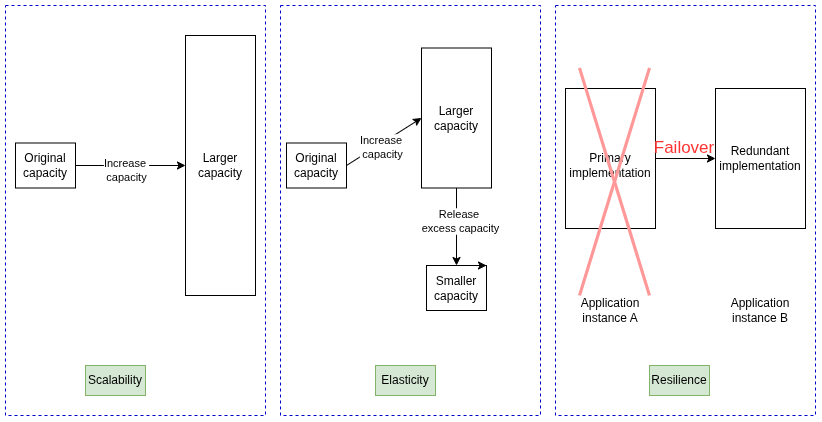
\includegraphics[width=1\linewidth]{images/part-a-1/PartA_1_imageCloudComputing.drawio.png.drawio.png}
    \caption{Conceptual comparison of scalability, elasticity and resilience}
    \label{fig:placeholder}
\end{figure}

\begin{table}[H]
\centering
\small
\renewcommand{\arraystretch}{1.3}

\begin{tabularx}{\textwidth}{
    @{}
    >{\raggedright\arraybackslash}p{0.22\textwidth}
    >{\raggedright\arraybackslash}X
    >{\raggedright\arraybackslash}X
    @{}
}
\toprule
\textbf{NIST essential characteristic}
&
\textbf{A local cluster}
&
\textbf{A grid}
\\
\midrule

\textbf{On-demand self-service}
&
\ding{55}: Users cannot directly provision computing and
storage resources themselves and generally require
administrator configuration.
&
\ding{55}: Resource allocation is controlled by the sites, not the user.
\\
\addlinespace

\textbf{Broad network access}
&
\ding{51}
&
\ding{51}
\\
\addlinespace

\textbf{Resource pooling}
&
\ding{51}
&
\ding{51}
\\
\addlinespace

\textbf{Rapid elasticity}
&
\ding{55}: The number of machines in a local cluster is fixed; adding or removing resources requires manual intervention by an administrator.
&
\ding{55}: Grid resources are distributed across institutional sites with no unified automatic scaling mechanism, and adding capacity may require coordination among institutions.
\\
\addlinespace

\textbf{Measured service}
&
\ding{55}: System logs alone do not necessarily provide complete
automatic resource metering, control and reporting.
&
\ding{55}: Quotas and queue records do not prove metering of actual resource usage
\\

\bottomrule
\end{tabularx}

\caption{Comparison of NIST Essential Characteristics in a Local Cluster and a Grid}
\label{tab:cluster-grid-nist}
\end{table}
